\chapter{User interface design}
\label{chap:user_interface_design}
\section{Method}
\label{sec:method}
We have chosen several different methods and processes that enable us to achieve results in a consistent manner. In this section, we will describe the methods we have applied, and explain why they were chosen over similar alternatives.

\subsection{Iterative design}
When designing a user interface with the intention of reaching a high level of usability, a systematic approach is key. The process we have used, can be roughly divided in to 4 steps, where the latter part can be repeated until the Quality Requirements, listed in \ref{subsec:quality_requirements}, have been met. \cite{lauesen} \\
The steps are:
\begin{enumerate}
\item Analysis of users and tasks
\item Construct prototype
\item Perform usability tests
\item Amend prototype 
\end{enumerate}

The semester planning and day to day booking have been described seperately, due to the differences between them. We will provide a detailed walkthrough of the process for an element in each part, and the full history of mockups can be found in appendix \ref{app:mockups}.

\subsection{Usability testing}
\label{sec:usability_testing}
With usability being our primary focus, choosing a proper method of testing said usability is key. A number of different variations of user-based testing exist:\cite{lauesen}
\begin{itemize}
\item \textbf{Observe only} - Let the user work out the task on his own, and simply observe his struggles
\item \textbf{Think aloud} - Let the users explain their thoughts and decision as they (try to) complete the tasks
\item \textbf{Cooperation} - Have two users solve the tasks together, and encourage them to discuss what is going on
\end{itemize}

Among the most widely used technique for testing user interfaces in development stages are the think aloud method.\cite{steve} As one can imagine, not all test subjects find it natural to explain their thoughts as they go, but with interested questions from the test evaluator, most users get familiar with the concept very fast. We have chosen the think aloud test for two primary reasons.
First, because even in the worst cases where a user does not adapt to explaining why and what they do, you can still get the same, if not better, results than with the \emph{observe only} test.
Secondly, the \emph{cooperation} test has the potential danger of concealing usability problems. In the case where test subjects \emph{t1} and \emph{t2} are cooperating on a task, a problem t1 would have encountered alone, will not be discovered due to p2 solving it beforehand, and vice versa. This results in potentially only finding problems which both users would have encountered on their own.

Surprisingly, we have not found any description of this problem by the established experts, and can therefore not verify our theory, but have nonetheless decided to avoid this version of usability testing, based on this. \\
\\
Choosing which, and how many, test subjects is needed for a test is a heavily debated subject in the usability community. Most tend to agree that 5 or below is more than enough for each round. The controversy arise when figuring out how representative the test subjects most be for your target audience. Soren Lauesen opens the corresponding chapter with: \cite{lauesen}
\begin{quotation}
\noindent \emph{``A usability test must of course be made with users that correspond to the real users we expect in practice.''}
\end{quotation}
However, Steve Krug has a different view: \cite{steve}
\begin{quotation}
\noindent \emph{``The importance of recruiting representative users is overrated. [...]''} \\
\noindent \emph{``The best-kept secret of usability testing is the extent to which it doesn't much matter who you test.''}
\end{quotation}

What we can take away from their different arguments for and against, is that testing with representative users is \emph{good}, but not vital when it simply comes to eliminating problems.
We have chosen to do both. The system is intended to be used by everyone at ITU, which will also include newly started students and faculty.
Another point of agreement among the experts, is that testing early and often will \emph{always} trump testing with many users at a later point. \cite{lauesen,steve,nielsen_five_users}

The table in figure \ref{fig:usa_users} shows how many users have been tested for each part of the system for each round. As seen, we've opted to only test one user for the semester planning, which is simply due to the lack of people with the required knowledge, and the very narrow target audience.

\begin{figure}[htb]
\begin{center}
\leavevmode
	\begin{tabular}{|l|r|r|r||r|}
		\hline
		 & Round 1 & Round 2 & Round 3 & Total \\ \hline
		Day to day & 2 & 2 & 2 & 6\\ \hline
		Semester & 1 & 1 & n/a & 2 \\ \hline
	\end{tabular}
\end{center}
\caption{Overview of test users per round}
\label{fig:usa_users}
\end{figure}


The results from our tests can be found in the following sections, whereas the full test documentation can be found in appendix \ref{app:tests}.

\section{Day to day booking}
\label{sec:day_to_day_booking_ui}
As described in previous chapters, the day to day booking should be usable without any instructions. We have tried to imitate familiar designs, and use common design conventions. As Steve Krug puts it\cite{steve}: 
\begin{quotation}
\emph{``All conventions start life as somebody's bright idea. If the idea works will enough, other sites imitate it and eventually enough people have seen it in enough places that it needs no explanation.''}
\end{quotation}

\subsection{Wireframe}
\label{subsec:wireframe}
The front page serves as a portal to the rest of the system, and thus it should be easy to understand. To ensure that we had the vital navigation functions in place before beginning the mockups, we constructed a wireframe\cite{garrett}. The wireframe, as seen on figure \ref{fig:wireframe_frontpage}, has the following elements:

\begin{figure}[htb]
\begin{center}
\leavevmode
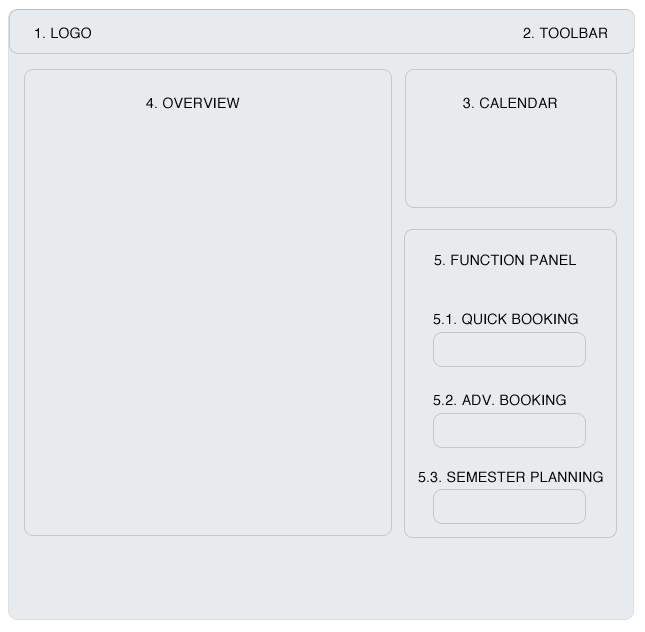
\includegraphics[width=0.6\textwidth]{images/wireframe1}
\end{center}
\caption{Wireframe for the frontpage}
\label{fig:wireframe_frontpage}
\end{figure}

\begin{itemize}
	\item \textbf{1. Logo}\\
	The logo for the application, which by convention should be located in the top left corner and link to the frontpage. \cite{steve}
	\item \textbf{2. Toolbar}\\
	A navigation toolbar. Should be used to login and logout, and for accessing the personal user account overview.
	\item \textbf{3. Calendar}\\
	An object used to navigate to a specific day in the future (or past).
	\item \textbf{4. Overview}\\
	The main overview, which should present a map of the university.
	\item \textbf{5. Function panel}\\
	A panel containing buttons used to enter the booking interface, or the semester planning.
\end{itemize}


\subsection{Test results}
\begin{figure}[htb]
\begin{center}
\leavevmode
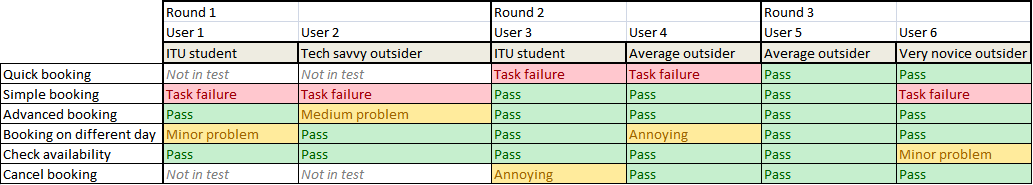
\includegraphics[width=1\textwidth]{images/result_day}
\end{center}
\caption{Test results for the day to day booking}
\label{fig:results_day}
\end{figure}

Figure \ref{fig:results_day} provides an overview of our findings from the usability testing of the day to day system. We have used the problem classification defined by Soren Lauesen\cite{lauesen}.

Reading the results, it becomes clear that we did not initially succeed in making vital functions of the system intuitive enough for users to utilize the indended functions. What may come as a surprise, is that most users at some point or the other, raised the complexity of the assigned task by accessing the advanced search function instead of the intended simpler functions.

What stands out here is that user 6 encountered two problems, one of which resulted in him not completing the assigned task. Naturally, this is not something we could wish for in the last round of testing, but it did provide insight as to how users with very little technical knowledge interpret our system.

The following section provides a walkthrough as to how a single part of the system have been designed, as direct results of the problems found in the test.

\subsection{Design process}
\label{sec:design_process}

\subsubsection{Design of the day to day booking interface}

For a full history of our mockups, please refer to %\ref{app:mockups_day} \\
\\

\begin{figure}[htb]
\begin{center}
\leavevmode
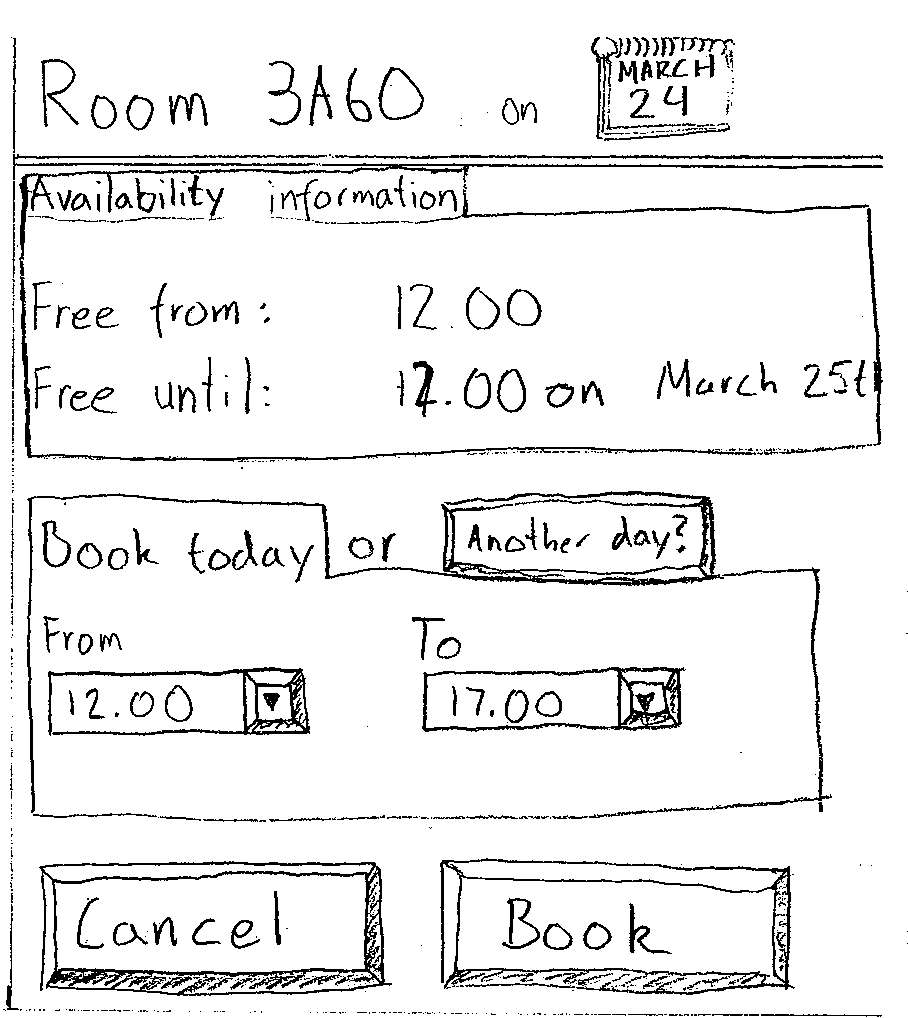
\includegraphics[width=0.6\textwidth]{images/bookRoomMockup}
\end{center}
\caption{First draft of the booking panel}
\label{fig:book_room_mockup}
\end{figure}

Seen on figure \ref{fig:book_room_mockup} is the function of the main screen, which was thought to be in charge of all interaction, trying to give the user the impression that they never left the homepage, and to make sure no-one got lost in subscreens and menus. Our first usability tests quickly revealed that we had been mistaken. All the test subjects felt overwhelmed by the amount of options, and due to all the clutter did not spot the vital functions.
\pagebreak
\begin{figure}[htb]
\begin{center}
\leavevmode
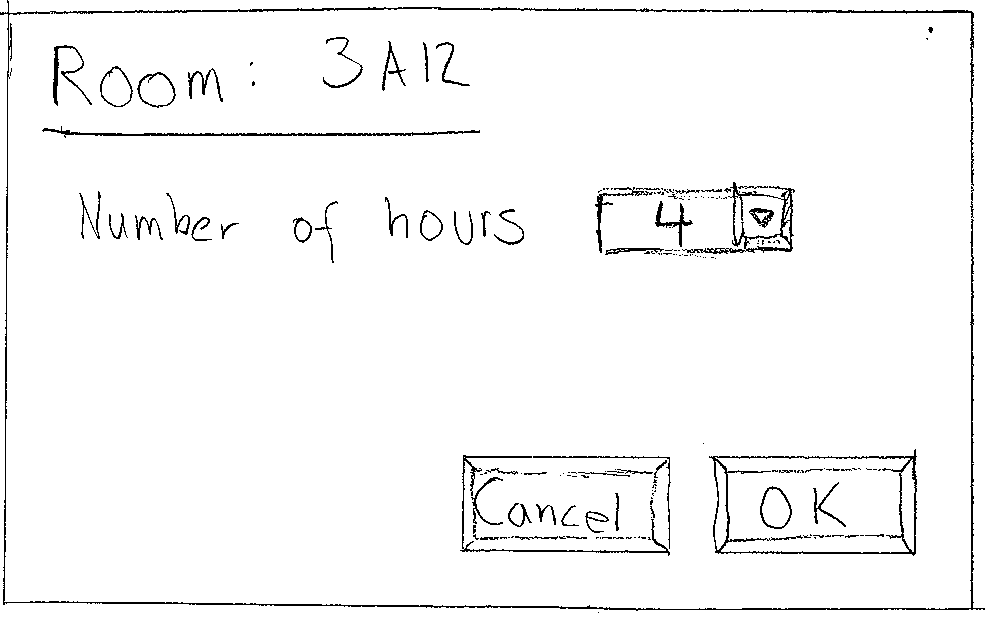
\includegraphics[width=0.8\textwidth]{images/bookRoomMockup2}
\end{center}
\caption{Second attempt at the simple booking. This time as a window overlaying the main view.}
\label{fig:book_room_mockup2}
\end{figure}

Second time around, we tried making it as basic as possible and simply presenting the user with a dialog (not a pop-up, just an overlay) for selecting how many hours from now the room should be booked. The flaw with this was that noone was able to figure out the availability of a room in the near future. This is when we realized that the best successes we've had with room booking was the first draft of the week-overview screen. \\
\\
This round of testing was probably the one with the biggest impact on the final design. As shown on the test results from figure \ref{fig:results_day}, \emph{quick booking} was not thought of yet in the first round. During the course of this test, we discovered general satisfaction with the simplicity of the overlaying panel even though it did not provide the needed functional for the intended task. However, we decided to find a new use for it, and that is how quick booking came to, along with simple booking being redefined to what it is now.

The result of this redefinition is described in section \ref{chap1:day_to_day_booking}. In summary, simple booking changed to become the interface used when clicking a room on the map view, whereas quick booking became the instant way of getting any available room.

\pagebreak
\begin{figure}[htb]
\begin{center}
\leavevmode
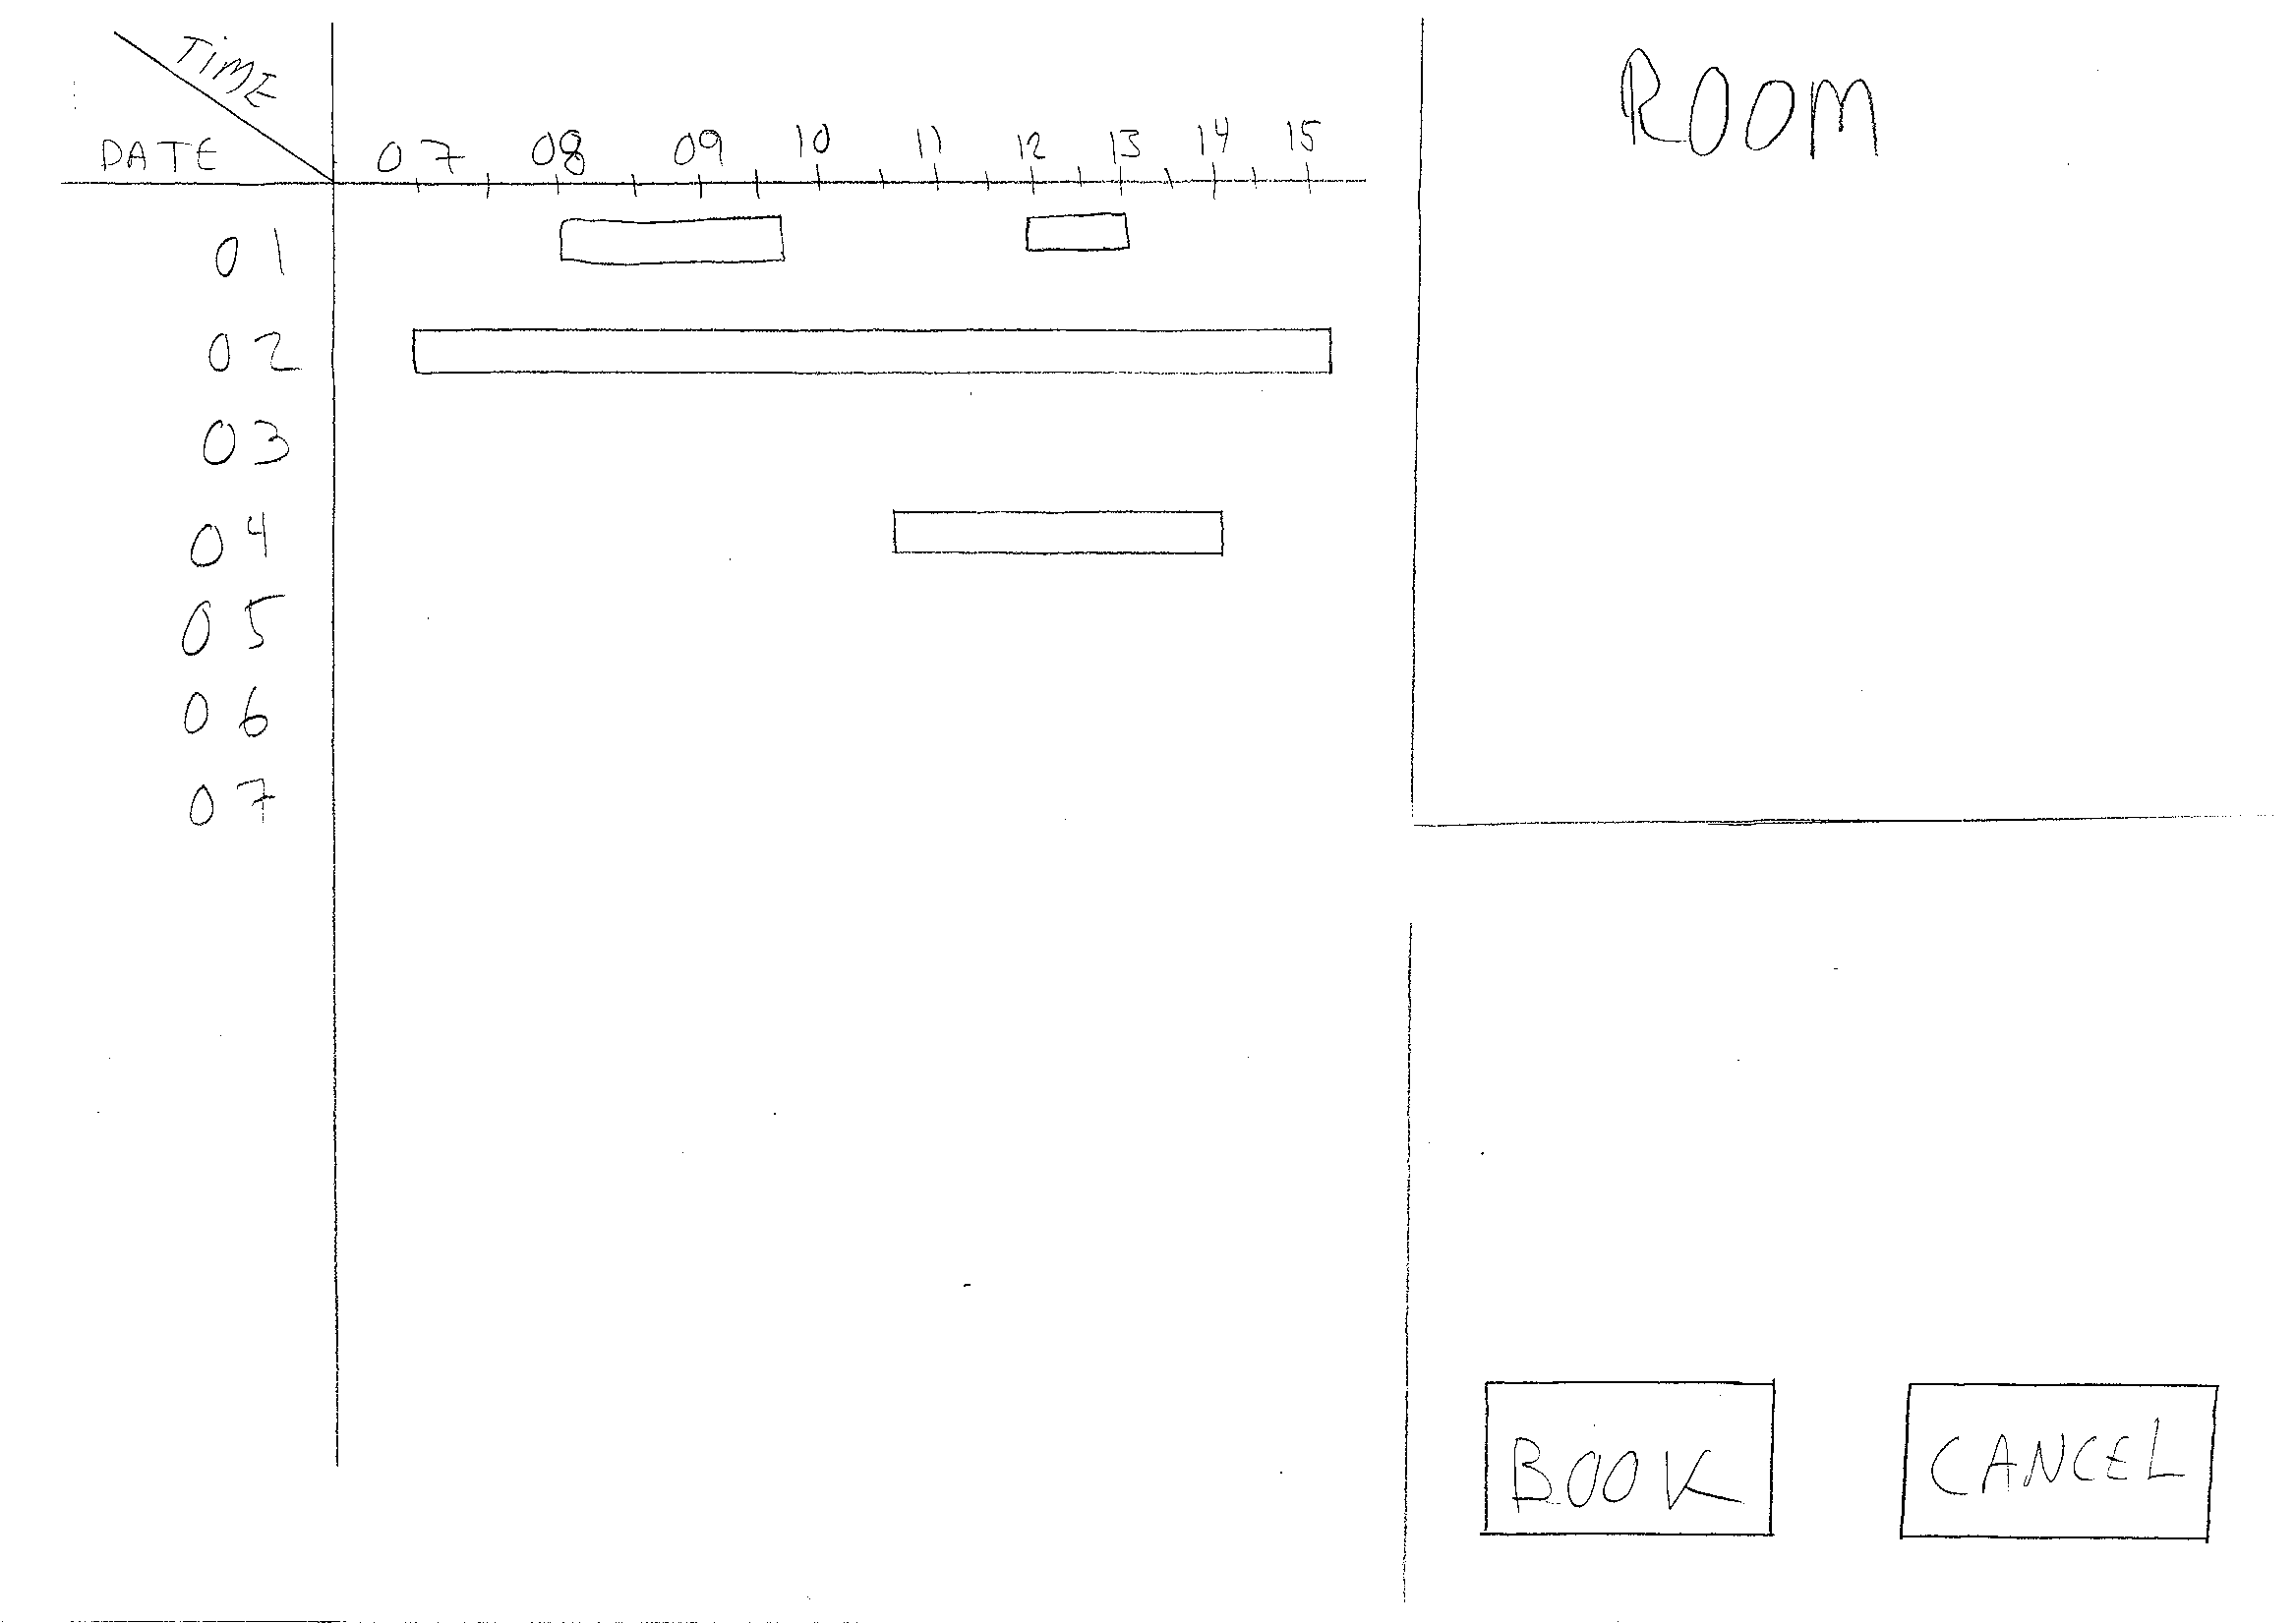
\includegraphics[width=0.8\textwidth]{images/weekMockup}
\end{center}
\caption{The mockup screen for a week overview on a specific room.}
\label{fig:week_mockup}
\end{figure}

All the test subjects used the 'matrix' overview shown on figure \ref{fig:week_mockup} both creatively and effectively, so we decided to try and utilize that success to the maximum by redirecting all bookings, bar the quick booking, to the same screen.

As shown, we have decided to invert the x/y-axes as opposed to normal day-time overviews in eg. Outlook or Google Calendar. This is done because of the standard timeline being from left to right, and not top to bottom. We have simply added 7 timelines on top of each, as we thought it more intuitive when trying to get an overview. Our assumptions proved correct from every single test, as not a single user had a problem understanding the view immediately.

\pagebreak
\begin{figure}[htb]
\begin{center}
\leavevmode
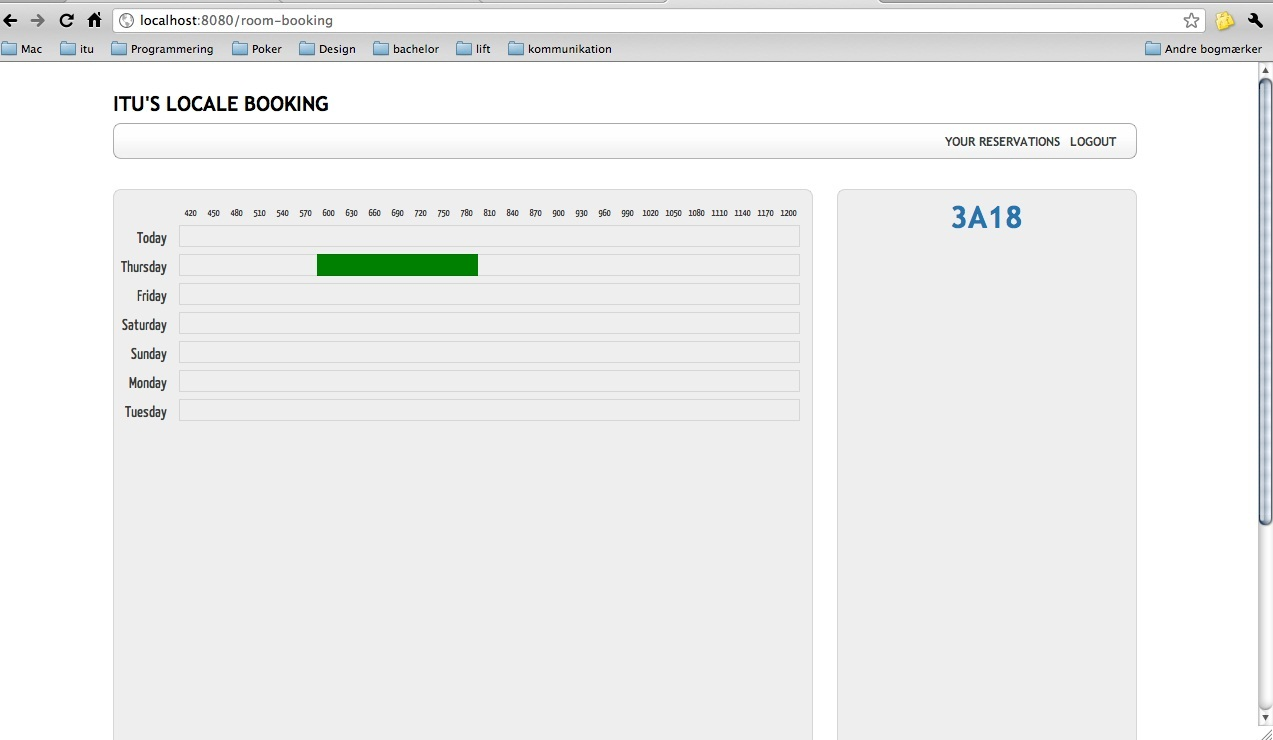
\includegraphics[width=1\textwidth]{images/weekFinal}
\end{center}
\caption{The finished screen for a week overview on a specific room, also used by Simple booking.}
\label{fig:week_final}
\end{figure}

The final design to book a room, as shown on figure \ref{fig:week_final}, grants an availability overview of 7 days, starting with the current day. Through our tests, we noted test subjects trying to drag the mouse to select, and others clicking for a start time followed by a click on end time, so we have chosen to allow for both.
To further assist the user in figuring out how it works, we have added highlighting of both the day and time when mouse is moved across the matrix.

The test results in figure \ref{fig:results_day} show a task failure for simple booking in last round, which was caused by him not discovering that the map was clickable, but once we intervened and directed him towards this view, he did succeed.


\subsection{Proposed design}
\label{sec:proposed_design}
\todo{Explain and illustrate the proposed design}

\section{Semester planning}
\label{sec:semester_planning_ui}
